\documentclass[t,xcolor={usenames,dvipsnames}]{beamer}

\mode<presentation>
{
\usetheme{Frankfurt}%{Warsaw}
%\setbeamercovered{transparent}
%\setbeamercolor{background canvas}{bg=white}
}

% Delete these, if you do not want the table of contents to pop up at
% the beginning of each (sub)section:
%\AtBeginSubsection[]
%{
%  \begin{frame}<beamer>{Outline}
%    \tableofcontents[currentsection,currentsubsection]
%  \end{frame}
%}
%\AtBeginSection[]
%{
%  \begin{frame}<beamer>{Outline}
%    \tableofcontents[currentsection]
%  \end{frame}
%}

\usepackage[english]{babel}
\usepackage[latin1]{inputenc}
\usepackage{times}
\usepackage[T1]{fontenc}
\usepackage{verbatim}
\usepackage{url}
\usepackage{amsmath,amssymb}
\usepackage{comment}
\usepackage{hyperref}

% Author-date citations
\usepackage[authoryear,round]{natbib}
\let\cite=\citep  % default \cite such as {\LaTeX} authors are used to

% Where \includegraphics should look for figures
\graphicspath{{./figs/}}
\usepackage{epstopdf}
\DeclareGraphicsExtensions{.eps,.png,.jpg,.pdf}

% Shortcuts
\newcommand{\myhref}[2]{\href{#1}{\textcolor{Blue}{#2}}}
\newcommand{\myurl}[1]{\myhref{#1}{#1}}
\newcommand{\subitem}[1]{\begin{itemize}[<.->]\item #1 \end{itemize}}
\newcommand{\ghead}[1]{{\tiny #1\\}}
\newcommand{\doi}[1]{\myhref{http://dx.doi.org/#1}{doi:#1}}
\newcommand{\csym}[1]{\textcolor{Blue}{\texttt{#1}}}


%%%%%%%%%%%%%%%%%%%%%%%%%%%%%%%%%%%%%%%%%%%%%%%%%%%%%%%%%%%%%%%%%%%%%%
\title{Life as a Research Software Engineer}
\author{Jonathan Cooper}
\institute[University of Oxford]
{Computational Biology Group\\
 Department of Computer Science\\
 University of Oxford}
\date{28\textsuperscript{th} January 2015}

\begin{document}

\begin{frame}
\titlepage
\end{frame}

%%%%%%%%%%%%%%%%%%%%%%%%%%%%%%%%%%%%%%%%%%%%%%%%%%%%%%%%%%%%%%%%%%%%%%

%\begin{frame}{Outline}
%\setcounter{tocdepth}{1}
%\tableofcontents
%\end{frame}

%%%%%%%%%%%%%%%%%%%%%%%%%%%%%%%%%%%%%%%%%%%%%%%%%%%%%%%%%%%%%%%%%%%%%%
\section{A brief history of me}
\subsection*{Main}
%%%%%%%%%%%%%%%%%%%%%%%%%%%%%%%%%%%%%%%%%%%%%%%%%%%%%%%%%%%%%%%%%%%%%%
% Start with personal slides v quickly as last done 2009/02/11 !
% And then again 2011/11/29...

\begin{frame}{1983 --- Tooting Bec, London}
\begin{columns}[T]
\column{.5\linewidth}
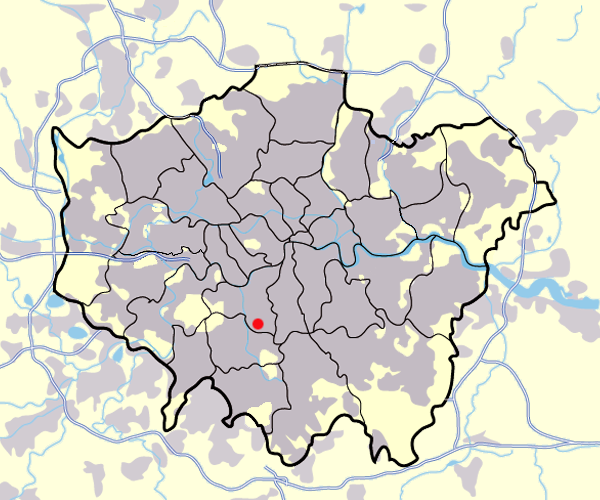
\includegraphics[width=.9\textwidth]{LondonMap}
\column{.5\linewidth}
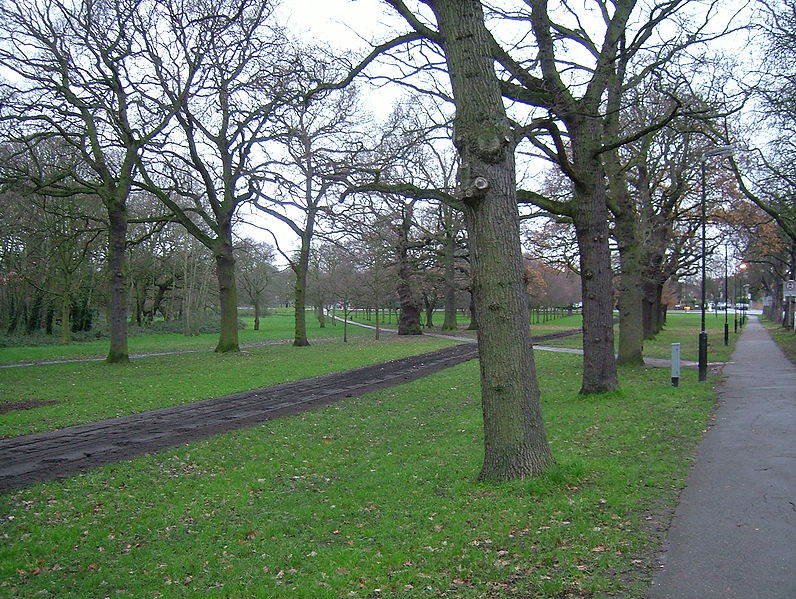
\includegraphics[width=.9\textwidth]{TootingBecCommon}
\end{columns}
\end{frame}

\begin{frame}{1987 --- Zambia, Africa}
\vspace{-1cm}
\begin{columns}[T]
\column{.5\linewidth}
\begin{center}
\only<1>{
\includegraphics[width=.9\textwidth]{ZambiaMap}}
\only<2>{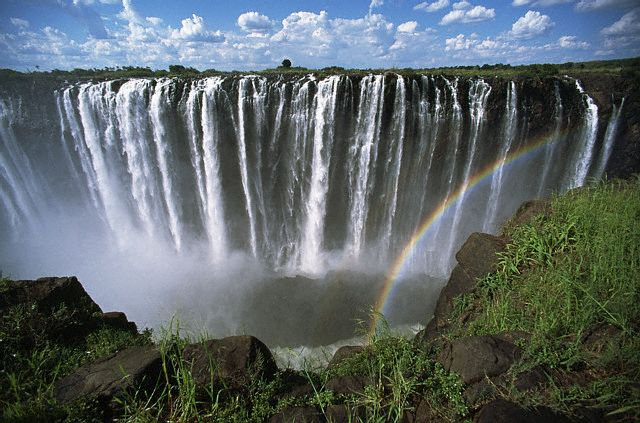
\includegraphics[width=.9\textwidth]{VictoriaFalls}\\
\vspace{.2cm}
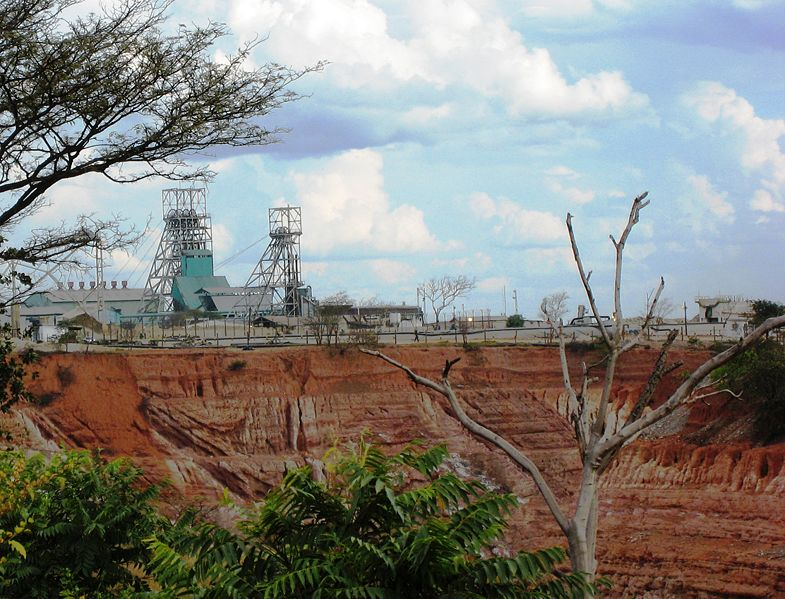
\includegraphics[width=.9\textwidth]{KitweCopperMine}}
\end{center}
\column{.5\linewidth}
\begin{center}
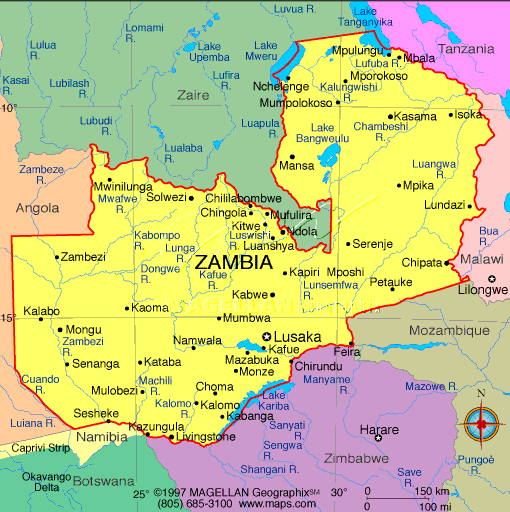
\includegraphics[width=.85\textwidth]{zambia}\\
\only<2>{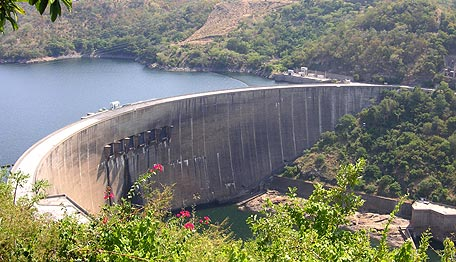
\includegraphics[width=.9\textwidth]{KaribaDam}}
\end{center}
\end{columns}
\end{frame}

\begin{frame}{1993 --- Back to England}
\begin{center}
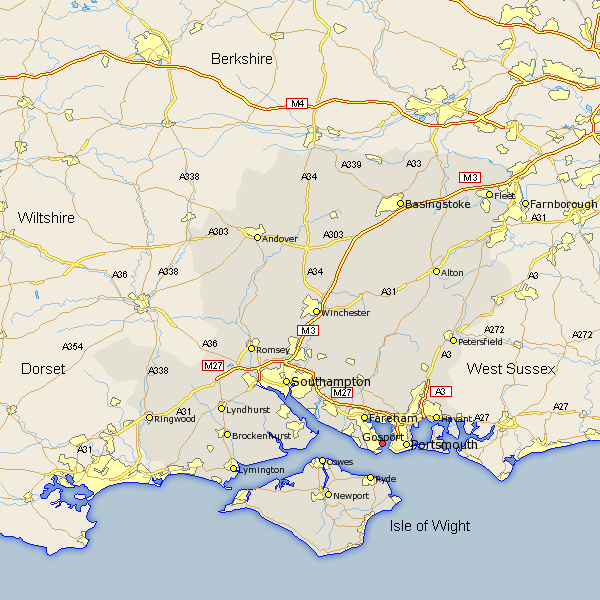
\includegraphics[height=.8\textheight]{GosportMap}
\end{center}
\end{frame}

\begin{frame}{2001 --- Oxford}
\begin{columns}[T]
\column{.33\linewidth}
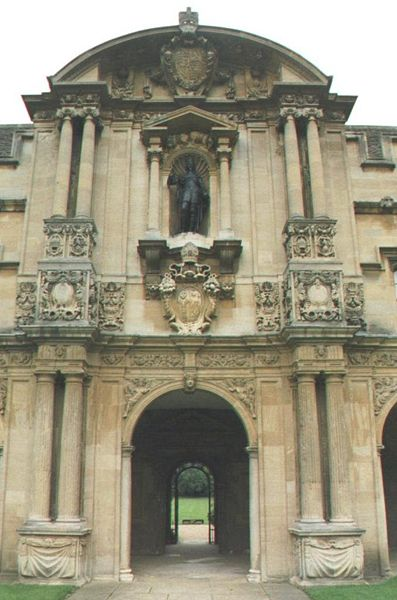
\includegraphics[width=.99\textwidth]{sjc1}
\column{.62\linewidth}
\hspace{.07\textwidth}
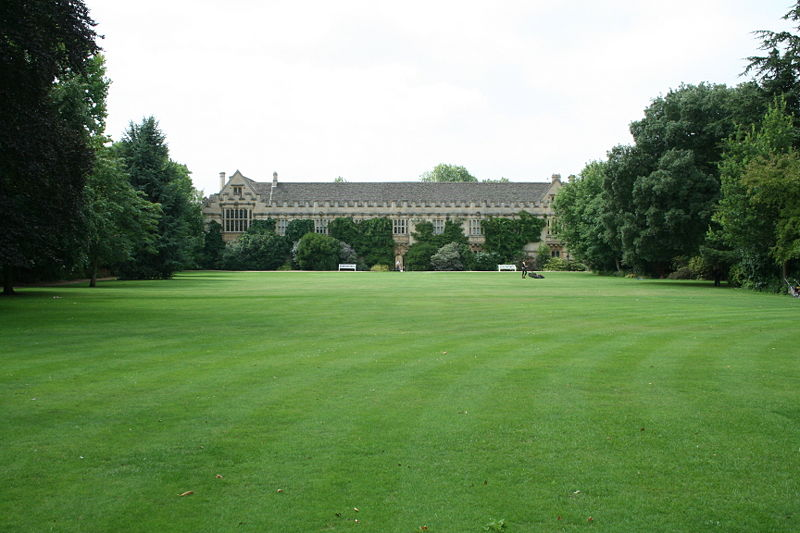
\includegraphics[width=.9\textwidth]{sjc2}
\begin{itemize}
\small
\item 2001: BA, Maths \& Computer Science
\item 2004: DPhil, LSI DTC \& Com Lab
\item 2008: Various postdocs
\item 2014: 50\% Assistant Director at SysBio DTC
\end{itemize}
\end{columns}
\end{frame}

%%%%%%%%%%%%%%%%%%%%%%%%%%%%%%%%%%%%%%%%%%%%%%%%%%%%%%%%%%%%%%%%%%%%%%
\section{Functional curation}
\subsection*{Main}
%%%%%%%%%%%%%%%%%%%%%%%%%%%%%%%%%%%%%%%%%%%%%%%%%%%%%%%%%%%%%%%%%%%%%%
% Brief intro to FC, focus on sell & concept
% Main themes of reproducibility & performance
% - comparing C++ & Python implementations
% - profiling & optimisation
% Tie in to RSE & numerics series; former is last main section

\begin{frame}{Improving the process of modelling}
\begin{itemize}[<2>]
\item As hypothesis encodings, models are developed \emph{for a specific purpose}
  \subitem{May not be appropriate for studying same system in different context}
\item How can we\ldots
  \begin{itemize}
  \item determine a model's functionality, i.e.\ its suitability or limitations for a new study? % Perhaps as part of a composite
  \item re-use a model in a different experimental context?
  \item compare hypotheses: different models' behaviours under the same experiment?
  \end{itemize}
\end{itemize}
\end{frame}


\begin{frame}{Functional curation with virtual experiments}
\vspace{-.2cm}
\subitem{Separate \alert{model structure} and \alert{experimental scenario}}
\vspace{-.2cm}
\hspace{-1cm}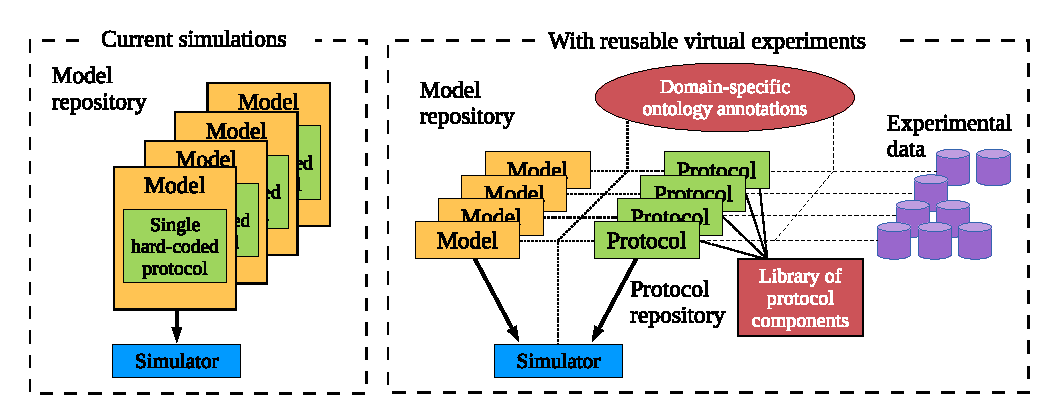
\includegraphics[width=1.185\textwidth]{virtual_expts_schematic}
\vspace{-.31cm}
\begin{itemize}
\item Apply any \alert{virtual experiment} to any (relevant) model
\item One definitive version of each model / protocol
\item Automatically generate post-processed outputs, plots, etc.
\end{itemize}
\end{frame}


\begin{frame}{Exemplar system: Cardiac electrophysiology}
\begin{center}
\vspace{-.5cm}
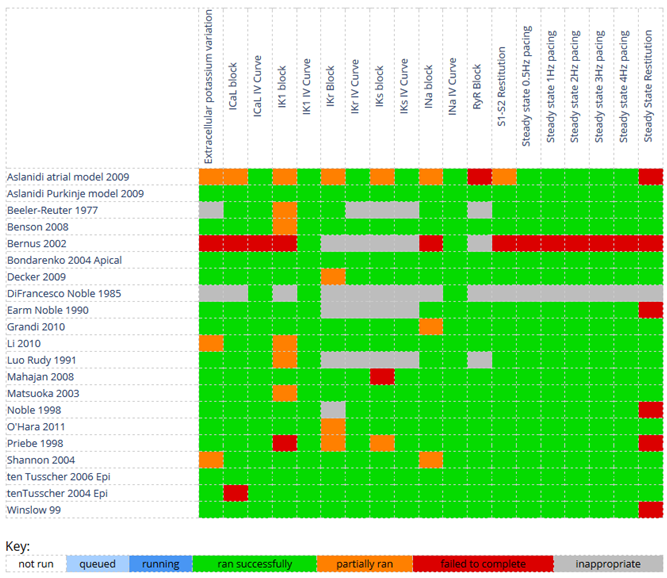
\includegraphics[height=.8\textheight]{cardiac_fc_matrix}\\
\myurl{https://chaste.cs.ox.ac.uk/FunctionalCuration}
\end{center}
\end{frame}


\begin{frame}{Results: regular pacing}
\begin{center}
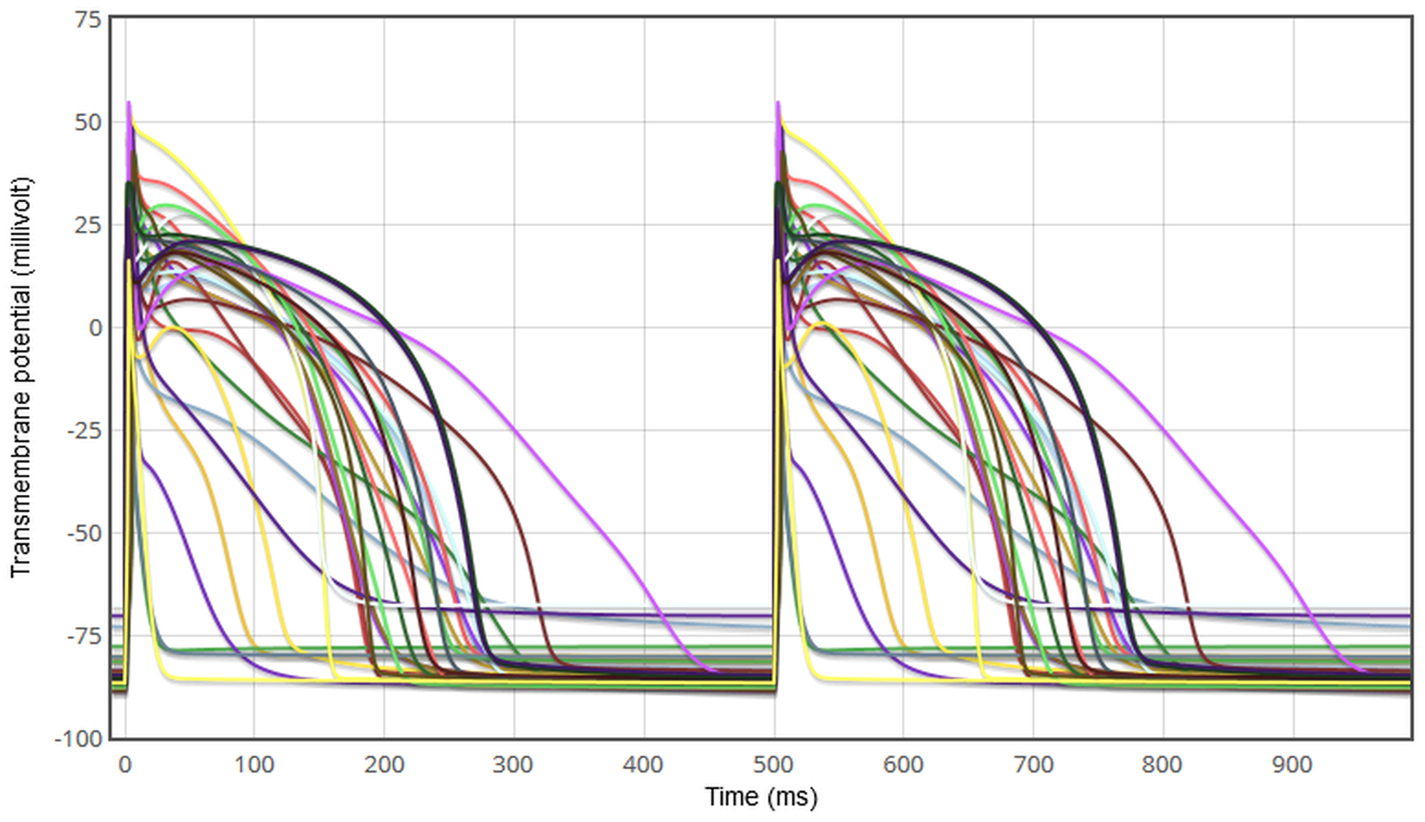
\includegraphics[width=\textwidth]{weblab_fig3}\\
\tiny\myurl{https://chaste.cs.ox.ac.uk/q/2014/fc/fig3}
\end{center}
\end{frame}


\begin{frame}{Results: restitution}
\begin{center}
\vspace{-.5cm}
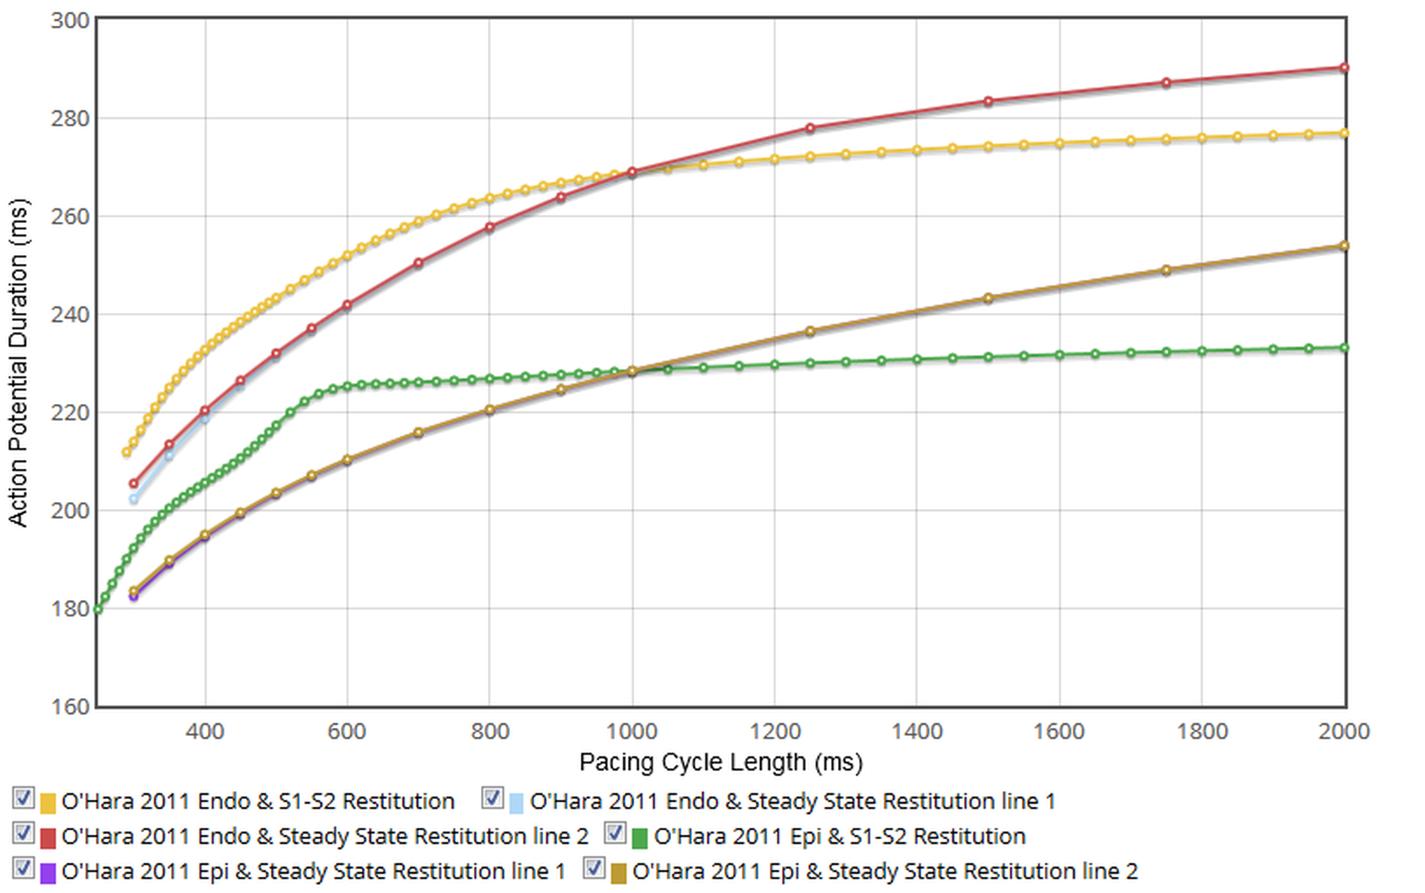
\includegraphics[width=\textwidth]{weblab_fig4}\\
\tiny\myurl{https://chaste.cs.ox.ac.uk/q/2014/fc/fig4}
\end{center}
\end{frame}


\begin{frame}{Results: drug block of NCX}
\begin{center}
\vspace{-.5cm}
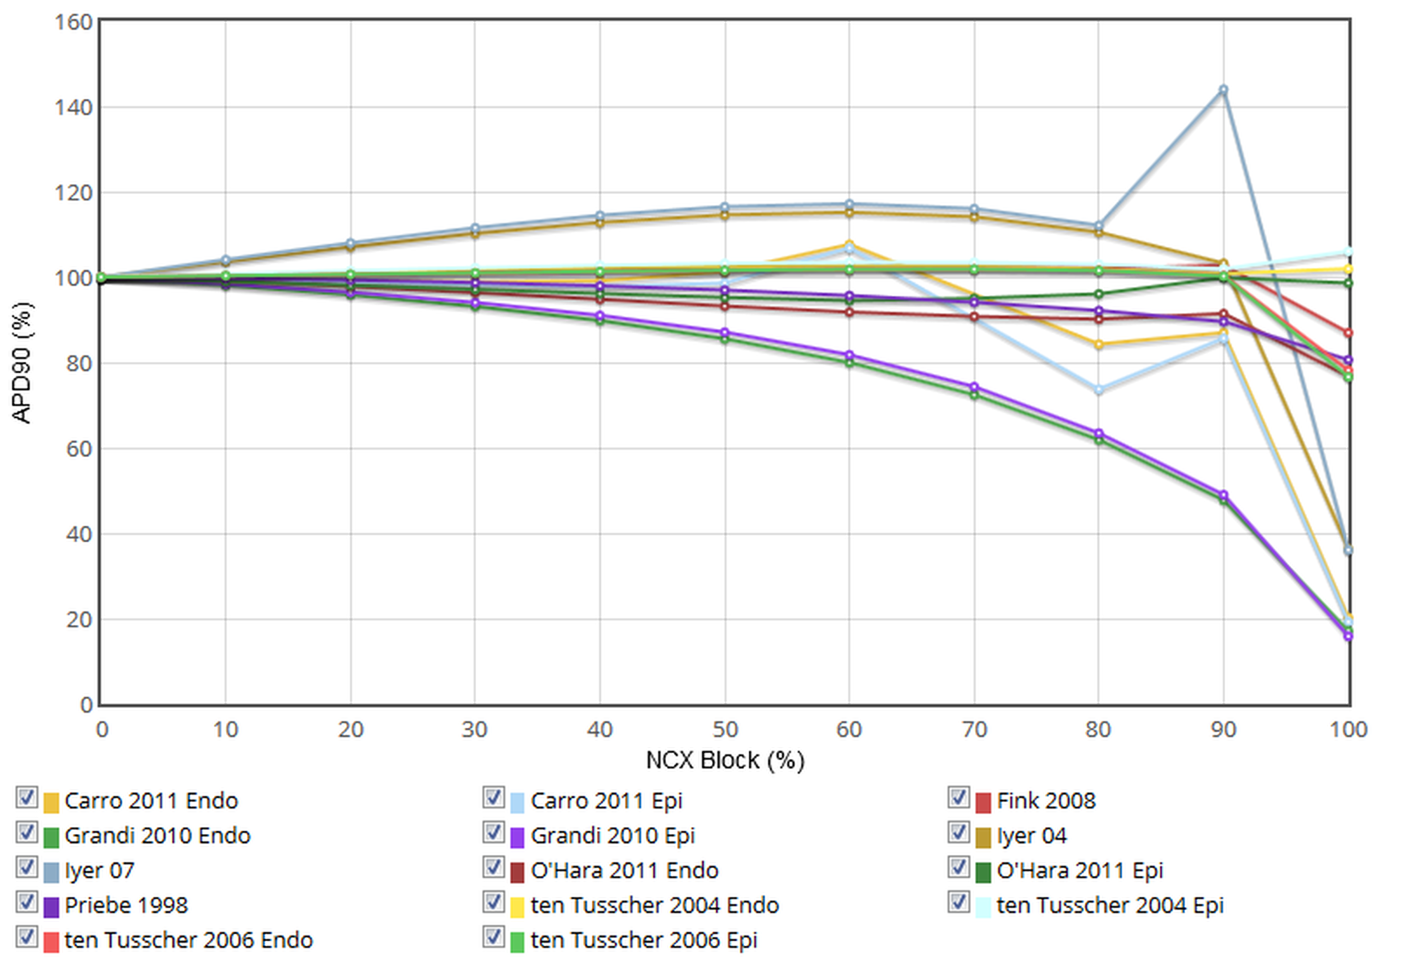
\includegraphics[width=\textwidth]{weblab_fig5}\\
\tiny\myurl{https://chaste.cs.ox.ac.uk/q/2014/fc/fig5}
\end{center}
\end{frame}


\begin{frame}{Results: steady state behaviour}
Priebe model under drug block of $I_{K_r}$.\\
\textbf{Left}: after just one pace at each degree of IKr block, these results are the same as those shown in Priebe et al. 1998.\\
\textbf{Right}: after 10000 paces for each degree of IKr block as shown in the Web Lab. Note that even the control action potential varies considerably, and is much longer in the steady state case.
\begin{center}
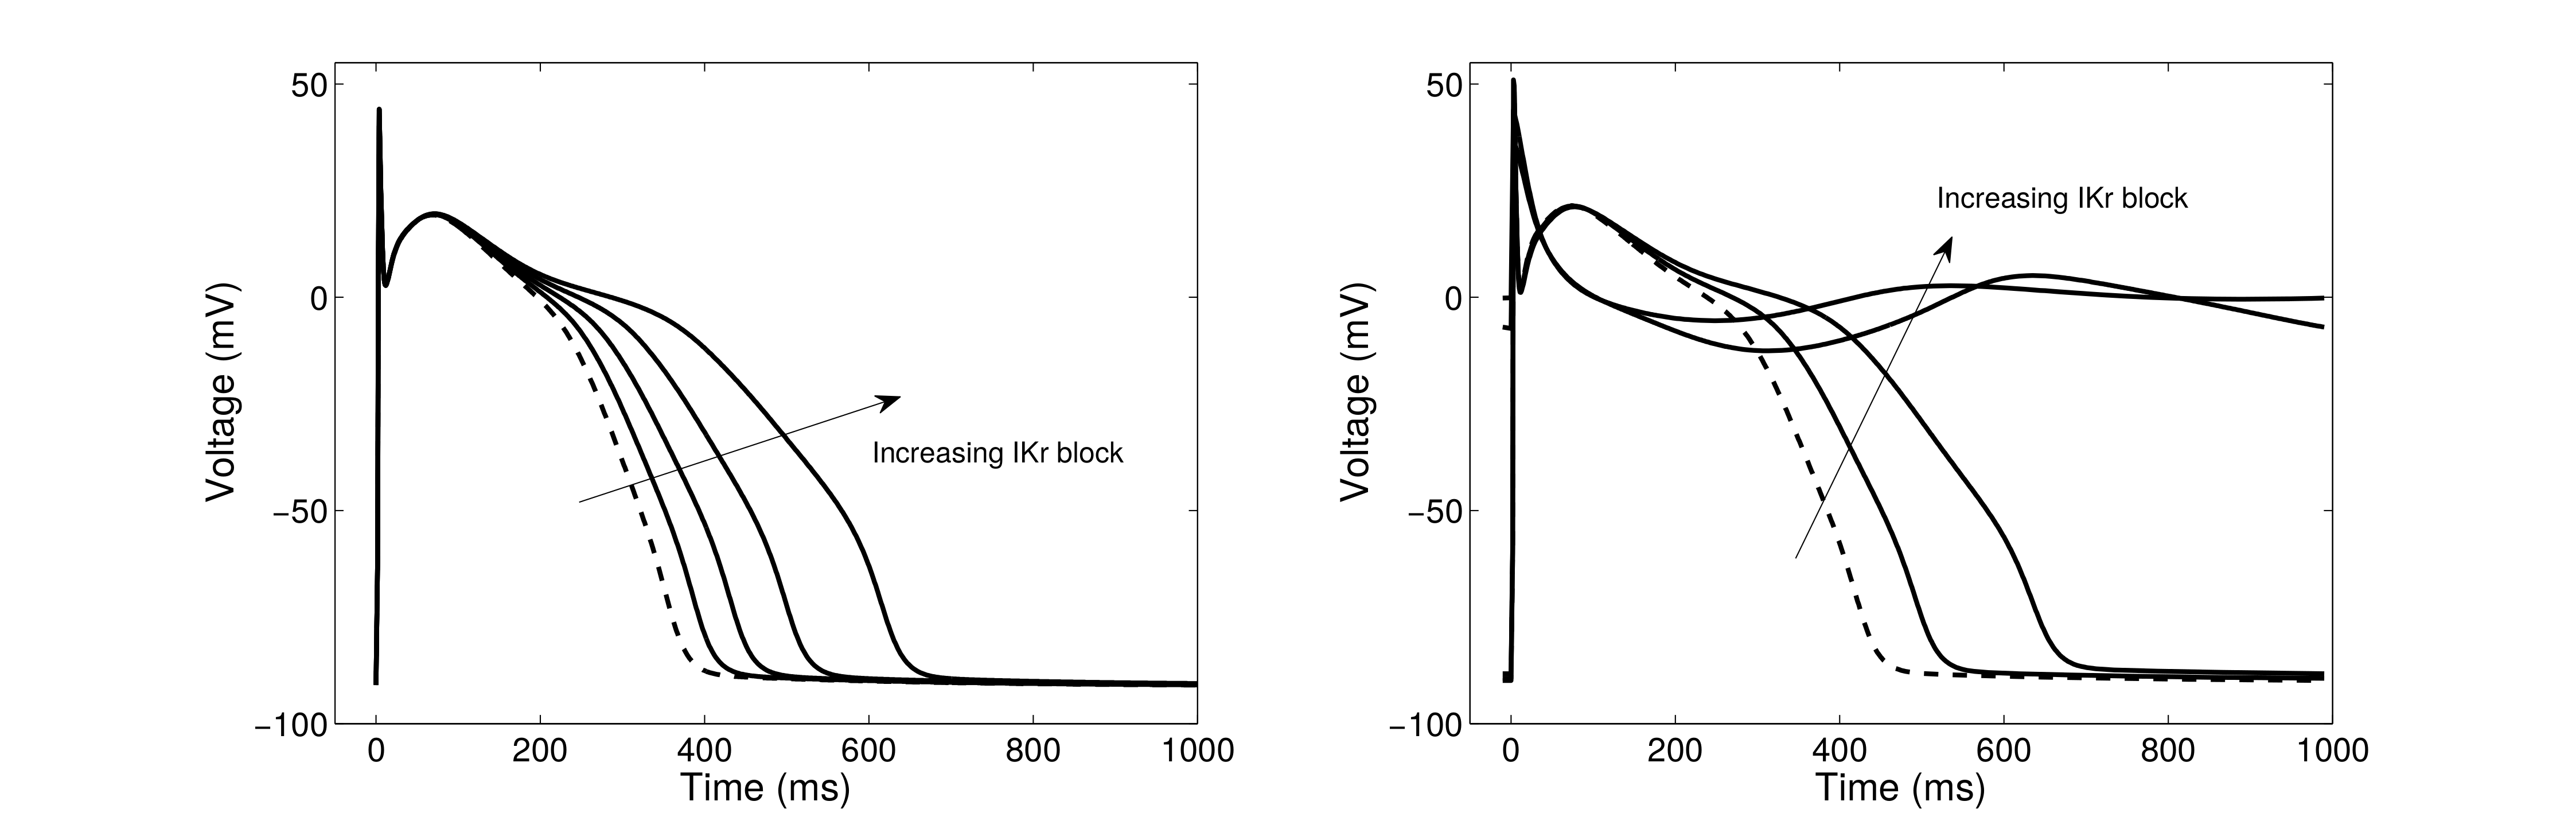
\includegraphics[width=\textwidth]{weblab_fig6}\\
\tiny\myurl{https://chaste.cs.ox.ac.uk/q/2014/fc/fig6}
\end{center}
\end{frame}


\begin{frame}{Results: fixing model encodings}
\begin{center}
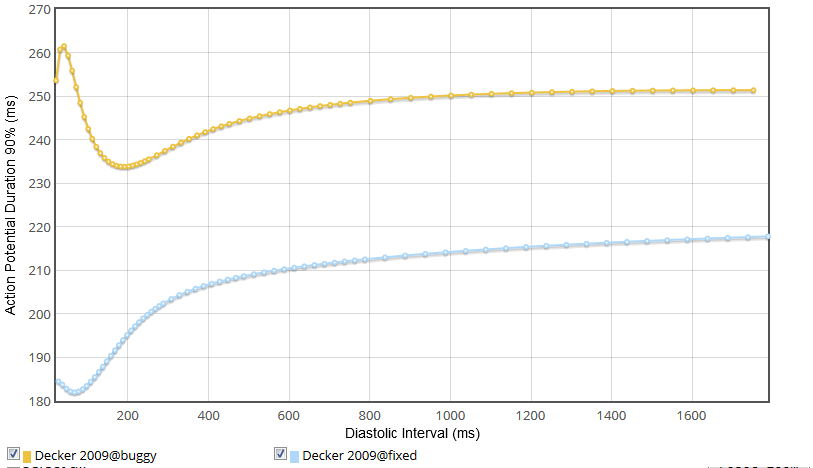
\includegraphics[width=\textwidth]{decker_comparison}

\tiny
\myurl{https://chaste.cs.ox.ac.uk/q/2014/fc/s1s2}

\myurl{https://chaste.cs.ox.ac.uk/q/2014/fc/diff}
\end{center}
\end{frame}

%%%%%%%%%%%%%%%%%%%%%%%%%%%%%%%%%%%%%%%%%%%%%%%%%%%%%%%%%%%%%%%%%%%%%%

\begin{frame}{What about reproducibility?}
Or, can you trust the results?
\begin{itemize}
\item The Web Lab stores all previously generated results
\item You can compare with previous versions of models, protocols and/or software
\item This isn't automatic
\item Separate test of the Chaste backend does automated regression testing of software
\end{itemize}
\end{frame}

%%%%%%%%%%%%%%%%%%%%%%%%%%%%%%%%%%%%%%%%%%%%%%%%%%%%%%%%%%%%%%%%%%%%%%

\begin{frame}{Python re-implementation: motivations}
The Web Lab backend is (mostly) C++ simulation code built on Chaste.\\
This is being re-implemented in Python.

\begin{itemize}[<2>]
\item Make it easier to extend what protocols can do
  \subitem{Especially more flexible post-processing and data structures}
\item Provide a basis for Aidan's parameter fitting work
\item Improve performance !
\end{itemize}
\end{frame}


\begin{frame}{Assessing performance}
\begin{itemize}
\item \alert{Profiling} identifies slow parts of code
\item Essential to profile before optimising
\item Chaste build system makes this (somewhat) easy
  % Show examples!  Explain how to interpret results.
\end{itemize}
\end{frame}


\begin{frame}{Profiling timeline}
\begin{tabular}{l|ll}
\textbf{Change summary} & \textbf{ICaL protocol} & \textbf{S1S2 protocol} \\
Original C++ code       & 197 (95)               & 201 (35) \\
\hline
Original Python code    & 792 (764)              & 279 (209) \\
Avoid CVODE resets      & 715                    & 270 \\
With Cython model       & 654                    & 224 \\
With extra cdefs        & 602 (573)              & 98 (34) \\
Avoid wrap/unwrap       & 438 (409)              & 96 (30) \\
Optimised SetVariable   & 361 (333)              & 98 (30) \\
Compile modifier exprs  & 264 (236)              & 97 (30) \\
Extra cdef in GetOutputs& 194 (167)              & 98 (30) \\
\hline
Avoid object creation   & 163 (135)              & 120 (28) \\
GetOutputs as list      & 159 (131)              & 119 (28) \\
Avoid a subtraction     & 147 (119)              & 118 (27) \\
\hline
Latest C++ code         & 264 (161)              & 202 (36) \\
\end{tabular}
\end{frame}


%%%%%%%%%%%%%%%%%%%%%%%%%%%%%%%%%%%%%%%%%%%%%%%%%%%%%%%%%%%%%%%%%%%%%%
\section{Research Software Engineering}
\subsection*{Main}
%%%%%%%%%%%%%%%%%%%%%%%%%%%%%%%%%%%%%%%%%%%%%%%%%%%%%%%%%%%%%%%%%%%%%%

\begin{frame}{Software for research}
\begin{itemize}
\item Software plays an increasingly fundamental role in today's research, but is not well supported by current structures.
\item In a recent SSI survey of Russell Group universities:
  \begin{itemize}
  \item 69\% of researches said their research would not be practical without software
  \item 56\% develop their own software
  \item Of those, \alert{21\%} have no training in software development
  \end{itemize}
\item How should software for science be developed?
  \begin{itemize}
  \item Scientists with better training
  \item Dedicated `Research Software Engineers' (RSEs)
  \end{itemize}
\end{itemize}
\end{frame}

\begin{frame}{What is needed at Oxford?}
\begin{itemize}
\item A \alert{network} allowing RSEs to share experiences and develop their skills, move more flexibly and reliably between grants, and build a \alert{career path} within the academic environment.
\item Provision of \alert{training for researchers} in how to think about software development in the right way, since much research software is naturally small-scale and problem-specific, and thus will need to be created by the researchers themselves.
\item Ultimately, a central team organising such training, and using a distributed team to provide \alert{software consultancy} more broadly than existing groups.
\end{itemize}
\end{frame}

\begin{frame}{Possible ways forward}
\begin{itemize}
\item Run more training activities for researchers
\item Develop a database of RSEs across the University
\item Build an RSE community
  \subitem{Community building, networking, professional development and support activities}
\item Lobby for a viable career path for RSEs within the University
  \subitem{Standard job title and description, recognition not based on publication record}
\item Lobby to set up a dedicated team (or teams) of RSEs to provide software consultancy and support across projects
\end{itemize}
\end{frame}

\begin{frame}{Current activities}
\begin{itemize}
\item In discussion with researchers across the sciences regarding best way forward
\item Working with digital humanities to identify and exploit commonalities
\item Read more at \myhref{http://goo.gl/HzUtSR}{goo.gl/HzUtSR}
\end{itemize}
\end{frame}

%%%%%%%%%%%%%%%%%%%%%%%%%%%%%%%%%%%%%%%%%%%%%%%%%%%%%%%%%%%%%%%%%%%%%%
\section{Conclusions}
\subsection*{Main}
%%%%%%%%%%%%%%%%%%%%%%%%%%%%%%%%%%%%%%%%%%%%%%%%%%%%%%%%%%%%%%%%%%%%%%

\begin{frame}{Conclusions}
\begin{itemize}
\item Performance doesn't always suffer where you might expect
\item Can you trust your code?
\item Talk to me if you are interested in Research Software Engineering!
\end{itemize}
\end{frame}


%%%%%%%%%%%%%%%%%%%%%%%%%%%%%%%%%%%%%%%%%%%%%%%%%%%%%%%%%%%%%%%%%%%%%%
\begin{frame}{Acknowledgments}
Gary Mirams, Aidan Daly\\
Chaste team\\

Web Lab: \myurl{https://chaste.cs.ox.ac.uk/FunctionalCuration}

\begin{center}

\includegraphics[scale=.9]{chaste-266x60}\\ \vspace{.3cm}

\includegraphics[scale=.7]{logo2020science}\\ \vspace{.4cm}

\includegraphics[width=.55\textwidth]{EPSRC1RGBLO} \hspace{.1cm}

\includegraphics[scale=.55]{logo_msr}
\end{center}
\end{frame}

\end{document}
